% ===========================================================================
% GravNet: Astrophysical Potential Dynamical Network (IEEEtran Formal Paper)
% 컴파일 명령어: cd docs && /Library/TeX/texbin/latexmk -xelatex gravnet_ieee.tex
% ===========================================================================
\documentclass[journal]{IEEEtran}

% ---------------------------------------------------------------------------
% 언어 및 한글 설정 (XeLaTeX + kotex)
% ---------------------------------------------------------------------------
\usepackage{kotex}
\setmainhangulfont{AppleMyungjo}[
  BoldFont={Apple SD Gothic Neo Bold},
  AutoFakeSlant=0.16
]
\setsanshangulfont{Apple SD Gothic Neo}[
  BoldFont={Apple SD Gothic Neo Bold},
  AutoFakeSlant=0.16
]
\setmonohangulfont{Apple SD Gothic Neo}

% ---------------------------------------------------------------------------
% 수식, 기호, 폰트 패키지
% ---------------------------------------------------------------------------
\usepackage{amsmath,amssymb,amsfonts,amsthm}
\usepackage{mathtools}
\usepackage{bm}

% ---------------------------------------------------------------------------
% 표 및 그래픽 패키지
% ---------------------------------------------------------------------------
\usepackage{graphicx}
\usepackage{booktabs}
\usepackage{tabularx}
\usepackage{array}
\usepackage{cite}
\usepackage{url}
\usepackage{xcolor}
\usepackage{tikz}
\usetikzlibrary{arrows.meta,positioning,shapes.geometric,calc,fit,backgrounds}

\graphicspath{{../GravNet/figures/}}

% ---------------------------------------------------------------------------
% 하이퍼링크 설정
% ---------------------------------------------------------------------------
\usepackage[colorlinks=true,linkcolor=black,urlcolor=blue,citecolor=black]{hyperref}

% ---------------------------------------------------------------------------
% 정리 및 보조정리 환경 정의
% ---------------------------------------------------------------------------
\newtheorem{theorem}{정리}
\newtheorem{lemma}{보조정리}
\newtheorem{definition}{정의}
\newtheorem{proposition}{명제}

% ---------------------------------------------------------------------------
% 제목 및 저자 정보
% ---------------------------------------------------------------------------
\title{시공간 중력장 궤도 신경망 (GravNet):\\플러머 퍼텐셜과 심플렉틱 궤도 역학을 이용한\\완전 무역전파 천체 분류}

\author{이인수}%
\thanks{본 연구의 모든 구현 코드, 기호 및 수치 검증 스크립트, 사전 학습된 모델 체크포인트 및 시각화 데이터는 공개 저장소 \url{https://github.com/yiinsu/stellar-classification}의 \texttt{GravNet/} 디렉토리에 수록되어 있다.}}

% 헤더 설정
\markboth{IEEE Transactions on Neural Networks and Learning Systems (Preprint), Vol.~XX, No.~X, November~2026}%
{Lee: 시공간 중력장 궤도 신경망 (GravNet)}

\begin{document}

\maketitle

% ---------------------------------------------------------------------------
% 영문 초록 및 색인어 (IEEE 표준 규격)
% ---------------------------------------------------------------------------
\begin{abstract}
Traditional deep neural networks rely heavily on layer-wise matrix multiplications and global backpropagation of error gradients, suffering from biological implausibility, non-convex gradient vanishing, and poor physical interpretability. In this paper, we propose \textbf{GravNet (Astrophysical Potential Dynamical Network)}, a novel first-principles dynamical learning paradigm that completely eliminates error backpropagation and backpropagation through time (BPTT). Instead of stacking discrete artificial layers, GravNet embeds input stellar observables into a $d$-dimensional fibered phase space $\mathbb{R}^d \times \mathbb{R}^d$ ($d=6$) and models celestial classification as an $N$-body orbital capture process governed by a multi-halo Plummer gravitational potential and symplectic dissipative Leapfrog dynamics. Every celestial particle launches strictly from the unclassified cosmic origin in a 2D equilateral supercluster plane via a multi-resolution spectral lens ($M=3,826$) combining geometric Doppler wavelets and Bochner random Fourier modes. Cosmic Hubble friction $\gamma > 0$ strictly guarantees monotonic Lyapunov mechanical energy dissipation ($dH/dt = -\gamma \|\mathbf{p}\|_2^2 \le 0$), capturing particles into class-specific Plummer basins within $T=10$ symplectic steps. Spacetime curvature and launch momenta are learned locally via contrastive mass sculpting and terminal tidal-force Hebbian plasticity without backward gradient propagation. Evaluated on the SDSS-17 benchmark (99,999 clean objects; 20,000 held-out test objects), a single-universe GravNet achieves an accuracy of \textbf{97.55\%} (Macro-$F_1$ \textbf{0.9718}) in 40.69 seconds of training, and a 3-universe multiverse achieves \textbf{97.59\%} (Macro-$F_1$ \textbf{0.9724}) with a \textbf{100.00\% recall (4,319/4,319)} on stars (\texttt{STAR}), outperforming backpropagation-trained MLPs (97.37\% / 97.42\%) and topology-evolving TWEANNs (97.45\%). Furthermore, GravNet naturally quantifies physical classification uncertainty via the Lagrange $L_1$ saddle-point potential barrier, achieving 98.71\% accuracy on deep-basin captures while physically isolating host-contaminated low-redshift quasars at the $L_1$ ridge.
\end{abstract}

\begin{IEEEkeywords}
GravNet, Non-backpropagation learning, Plummer potential, Symplectic integrator, Lyapunov stability, Lagrange $L_1$ saddle points, SDSS-17 stellar classification.
\end{IEEEkeywords}

% ---------------------------------------------------------------------------
% I. 서론
% ---------------------------------------------------------------------------
\section{서론 (Introduction)}
\IEEEPARstart{현}{대} 딥러닝(Deep Learning)의 패러다임은 이산적인 은닉층(Hidden Layer)의 가중치 행렬곱과 활성화 함수 합성, 그리고 연쇄법칙(Chain Rule)에 기반한 전역 오차 역전파(Backpropagation, BP)에 확고히 뿌리를 두고 있다~\cite{yosinski2014}. 그러나 역전파 알고리즘은 생물학적 신경계의 국소 시냅스 가소성과 불일치하는 전치 가중치 전송 문제(Weight Transport Problem)를 지니며, 시계열 및 연속 동역학 최적화 시 시간 역전파(Backpropagation Through Time, BPTT)의 높은 메모리 소모와 기울기 소실·폭발 문제를 동반한다~\cite{hinton2022,scellier2017}.

더욱이 천체물리학(Astrophysics) 도메인의 천체 분류 과제---슬론 디지털 전천 탐사(Sloan Digital Sky Survey, SDSS-17)의 5개 측광 등급($u, g, r, i, z$), 색지수, 그리고 분광 적색편이($z$, \texttt{redshift})로부터 은하(\texttt{GALAXY}), 퀘이사(\texttt{QSO}), 별(\texttt{STAR})을 판별하는 문제---에서 정적 인공 신경망은 관측 대상이 본질적으로 시공간 속을 비행하는 물질과 전자기파라는 물리적 실체를 반영하지 못한다.

앞서 본 연구진이 구축한 기준선 파이프라인 중 전역 역전파 기반 다층 퍼셉트론(\texttt{DL/}, 단일 모델 $97.37\%$, 3-Seed 앙상블 $97.42\%$)과 유전적 구조 변이를 적용한 위상·가중치 진화 신경망(\texttt{EDL/TWEANN}, 단일 챔피언 $97.43\%$, 상위 4섬 앙상블 $97.45\%$)~\cite{stanley2002}은 우수한 성과를 보였으나, 여전히 정적 계산 그래프라는 틀을 벗어나지 못했다.

본 논문에서는 천체역학(Astrodynamics)과 비평형 통계물리학의 제1원리(First Principles)로부터 출발하는 완전히 새로운 학습 모델인 \textbf{시공간 중력장 궤도 신경망(Astrophysical Potential Dynamical Network, 코드명 \texttt{GravNet})}을 제안한다. \texttt{GravNet}은 은닉층을 완전히 배제하고, 입력 별빛을 고차원 위상 공간(Phase Space)에 발사된 시험 입자(Test Particle)로 모델링하여 구상성단과 은하 암흑물질 헤일로의 밀도 분포를 설명하는 \textbf{플러머 중력 퍼텐셜(Plummer Potential)}~\cite{plummer1911} 지형 속에서 스스로 궤도 운동을 수행하게 만든다.

본 연구의 핵심 기여는 다음과 같다:
\begin{enumerate}
  \item \textbf{완전 무역전파(100\% Backpropagation-Free) 물리 학습}: 궤도 적분에 대한 시간 역전파(BPTT)를 전혀 사용하지 않고, 1단계 닫힌 해 숄레스키 발사 보정, 2단계 대조적 시공간 곡률 조각 및 종착 조석력 벡터($\mathbf{f}_{\text{tidal}}$) 기반 헤비안 렌즈 가소성, 3단계 대정준 화학 퍼텐셜 보정의 3단계 순수 물리 학습 법칙을 정립하였다.
  \item \textbf{리아푸노프 단조 소산 정리 및 엄밀성 증명}: 허블 우주 마찰 $\gamma > 0$이 결합된 대칭 스트랭 분할(Strang-Split) 심플렉틱 리프프로그 적분기에서 기계적 총 해밀토니안의 단조 소산($dH/dt = -\gamma \|\mathbf{p}\|_2^2 \le 0$)을 수학적으로 증명하고, \texttt{SymPy} 기호 미분과 2차 유한차분($\text{Error} < 1.84 \times 10^{-10}$)으로 해석적 일치성을 검증하였다.
  \item \textbf{벤치마크 최고 성능 달성}: 20,000건 테스트 세트에서 단일 우주 \texttt{GravNet}이 \textbf{97.55\%} (Macro-$F_1$ \textbf{0.9718}), 3-우주 다중우주가 \textbf{97.59\%} (Macro-$F_1$ \textbf{0.9724})를 기록하여 역전파 딥러닝과 진화 신경망을 모두 넘어섰으며, 항성(\texttt{STAR}) 4,319개를 단 한 건의 오차도 없이 \textbf{100.00\% 재현율(4,319/4,319)}로 포획하였다.
  \item \textbf{라그랑주 $L_1$ 안장점 기반 물리적 불확실성 분리}: 두 은하단 중력이 비기는 라그랑주 $L_1$ 퍼텐셜 장벽 $\Delta E_{L_1}$을 통해, 별도의 베이지안 모듈 없이도 깊은 우물 포획군(상위 95\%)에서 \textbf{98.71\%}의 초고정밀도를 달성함과 동시에 모은하 빛이 섞인 저적색편이 퀘이사 경계군을 물리적으로 분리해 냈다.
\end{enumerate}

% ---------------------------------------------------------------------------
% II. 이론적 배경 및 물리 동역학 정식화
% ---------------------------------------------------------------------------
\section{이론적 배경 및 물리 동역학 정식화}

\subsection{섬유 다발 위상 공간과 다중 해상도 천체 분광 렌즈}
입력 천체 관측 벡터 $\mathbf{x} \in \mathbb{R}^{d_{\text{in}}}$ ($d_{\text{in}} = 10$)는 5개 측광 등급, 적색편이 $z$, 그리고 4개 색지수로 구성된다. 이를 단위 질량($m = 1$) 시험 입자의 위상 공간 $\mathcal{P} = \mathbb{R}^d \times \mathbb{R}^d$ ($d = 6$) 상태 벡터 $(\mathbf{q}(t), \mathbf{p}(t))$로 사상한다. 위치 좌표 공간 $\mathbb{R}^6$은 직합 구조를 갖는다:
\begin{equation}
  \mathbf{q}(t) = \big(\mathbf{q}_{\text{orb}}(t),\, \mathbf{q}_{\text{spec}}(t)\big) \in \mathbb{R}^2 \oplus \mathbb{R}^4.
  \label{eq:phase_space_decomp}
\end{equation}
$\mathbf{q}_{\text{orb}}(t) \in \mathbb{R}^2$는 세 천체 종족의 거대 초은하단 중심 $\mathbf{S}_c \in \mathbb{R}^6$ ($c \in \{0, 1, 2\}$)가 반지름 $R_{\text{sc}} = 3.2$, 각도 $\theta_c \in \{\frac{\pi}{2}, \frac{7\pi}{6}, \frac{11\pi}{6}\}$ ($120^\circ$ 정삼각형 대칭)로 배치된 \textbf{2차원 초은하단 궤도 평면}이며, $\mathbf{q}_{\text{spec}}(t) \in \mathbb{R}^4$는 클래스 내부의 미세 아종을 식별하는 \textbf{4차원 분광 섬유(Spectral Fiber)}이다.

극단적 이상치에 대한 완충을 위해 $\tilde{\mathbf{x}} = 15 \tanh(\mathbf{x}/15)$를 취한 뒤, 보크너 정리(Bochner's Theorem)~\cite{rahimi2007}에 기반한 \textbf{다중 해상도 분광 렌즈} $\Phi(\mathbf{x}) \in \mathbb{R}^M$ ($M = 3,826$)를 정의한다:
\begin{equation}
\begin{aligned}
  \Phi(\mathbf{x}) = \Big[\, &1 \;\Big\Vert\; \tilde{\mathbf{x}}^\top \;\Big\Vert\; \tfrac{1}{4}\big(\tilde{x}_i \tilde{x}_j\big)_{1 \le i \le j \le 10} \;\Big\Vert\; \tfrac{1}{\sqrt{F}}\sin(\tilde{\mathbf{x}} \otimes \boldsymbol{\omega}_{\text{1D}}) \\
  &\Big\Vert\; \tfrac{1}{\sqrt{F}}\cos(\tilde{\mathbf{x}} \otimes \boldsymbol{\omega}_{\text{1D}}) \;\Big\Vert\; \sqrt{\tfrac{2}{M_{\text{RFF}}}}\cos(\tilde{\mathbf{x}}^\top \boldsymbol{\Omega} + \boldsymbol{\varphi}^\top) \,\Big]^\top.
\end{aligned}
\end{equation}
여기서 $\boldsymbol{\omega}_{\text{1D}} \in \mathbb{R}^F$ ($F = 44$)는 $z \approx 0$ 근방의 미세 도플러 경계를 포착하기 위해 $\omega_{\min} = 0.25$부터 $\omega_{\max} = 120.0$까지 로그 스케일로 배치된 1차원 조화 기저이며, $\boldsymbol{\Omega} \in \mathbb{R}^{10 \times M_{\text{RFF}}}$ ($M_{\text{RFF}} = 2,880$)는 다중 대역폭 가우시안 측도에서 추출된 비등방성 무작위 푸리에 주파수 행렬이다.

\begin{definition}[우주 원점 발사 조건]
발사 행렬 $\mathbf{W}_q \in \mathbb{R}^{M \times 6}$의 궤도 평면 성분은 영행렬($[\mathbf{W}_q]_{:, 1:2} = \mathbf{0}$)로 구속된다. 즉, 모든 입자는 초기 시각 $t=0$에서 초은하단 궤도 평면의 미분류 원점 $(0, 0)$에서 출발한다:
\begin{align}
  \mathbf{q}_{\text{orb}}(0) &= \mathbf{0}_2, \quad \mathbf{q}_{\text{spec}}(0) = \Phi(\mathbf{x})^\top [\mathbf{W}_q]_{:, 3:6}, \nonumber \\
  \mathbf{p}(0) &= \Phi(\mathbf{x})^\top \mathbf{W}_p.
  \label{eq:launch_origin}
\end{align}
\end{definition}

\subsection{다중 헤일로 플러머 퍼텐셜 및 해석적 중력장}
특이점($r \to 0$) 발산을 방지하기 위해 천체물리학의 구상성단 모델인 플러머 퍼텐셜(Plummer Potential)~\cite{plummer1911}을 도입한다. 각 클래스 $c$마다 $K = 6$개의 플러머 중력 핵 위치 $\boldsymbol{\mu}_{c,m} \in \mathbb{R}^d$와 양의 중력 질량 $G_{c,m} > 0$ (총 $3K = 18$개 중력원)이 존재하며, 우주 조화 가둠 계수 $\kappa > 0$, 연화 길이 $\epsilon > 0$ 하에서 총 퍼텐셜 $U(\mathbf{q})$는 다음과 같다:
\begin{equation}
  U(\mathbf{q}) = -\sum_{c=0}^{2}\sum_{m=1}^{K} \frac{G_{c,m}}{\sqrt{\|\mathbf{q} - \boldsymbol{\mu}_{c,m}\|_2^2 + \epsilon^2}} + \frac{1}{2}\kappa \|\mathbf{q}\|_2^2.
  \label{eq:total_potential}
\end{equation}

$\epsilon > 0$이므로 $U \in C^\infty(\mathbb{R}^d)$이며, 편미분을 전개하여 얻어지는 닫힌 수식의 중력장 $\mathbf{F}_{\text{grav}}(\mathbf{q}) = -\nabla_{\mathbf{q}} U(\mathbf{q})$는 자동미분 없이 즉시 계산된다:
\begin{equation}
  \mathbf{F}_{\text{grav}}(\mathbf{q}) = -\sum_{c=0}^{2}\sum_{m=1}^{K} G_{c,m} \frac{\mathbf{q} - \boldsymbol{\mu}_{c,m}}{\left(\|\mathbf{q} - \boldsymbol{\mu}_{c,m}\|_2^2 + \epsilon^2\right)^{3/2}} - \kappa \mathbf{q}.
  \label{eq:analytic_force}
\end{equation}

\subsection{리아푸노프 에너지 소산 정리와 심플렉틱 적분}
허블 마찰 계수 $\gamma > 0$가 결합된 감쇠 해밀턴 운동 방정식은 다음과 같다:
\begin{equation}
  \dot{\mathbf{q}} = \mathbf{p}, \qquad \dot{\mathbf{p}} = -\nabla_{\mathbf{q}} U(\mathbf{q}) - \gamma \mathbf{p}.
  \label{eq:damped_eom}
\end{equation}

\begin{theorem}[리아푸노프 단조 소산 및 평형점 수렴성]
$\epsilon > 0, G_{c,m} > 0, \kappa > 0, \gamma > 0$일 때, 총 역학적 해밀토니안 $H(\mathbf{q}, \mathbf{p}) = \frac{1}{2}\|\mathbf{p}\|_2^2 + U(\mathbf{q})$는 아래로 유계이고 방사 강제성을 가지며, 궤적을 따라 단조 감소하여 모든 해는 정지 평형점 집합 $\mathcal{E} = \{(\mathbf{q}^*, \mathbf{0}) \mid \nabla_{\mathbf{q}} U(\mathbf{q}^*) = \mathbf{0}\}$으로 수렴한다.
\end{theorem}

\begin{IEEEproof}
$\sqrt{\|\mathbf{q}-\boldsymbol{\mu}_{c,m}\|_2^2+\epsilon^2} \ge \epsilon$이므로 $H(\mathbf{q}, \mathbf{p}) \ge \frac{1}{2}\|\mathbf{p}\|_2^2 + \frac{1}{2}\kappa\|\mathbf{q}\|_2^2 - \frac{1}{\epsilon}\sum_{c,m}G_{c,m} > -\infty$이다. $\kappa > 0$이므로 $\|(\mathbf{q}, \mathbf{p})\|_2 \to \infty$일 때 $H \to +\infty$가 되어 모든 부분준위집합 $\Omega_c$는 콤팩트 집합이다. 시간 도함수를 전개하면
\begin{equation}
\begin{aligned}
  \frac{dH}{dt} &= \langle \nabla_{\mathbf{q}} U, \mathbf{p} \rangle + \langle \mathbf{p}, -\nabla_{\mathbf{q}} U - \gamma \mathbf{p} \rangle \\
  &= -\gamma \|\mathbf{p}\|_2^2 \le 0.
\end{aligned}
\end{equation}
$\dot{H} = 0 \iff \mathbf{p} = \mathbf{0}$이다. 최대 불변 집합 내에서 $\mathbf{p} \equiv \mathbf{0} \implies \dot{\mathbf{p}} \equiv \mathbf{0}$이므로 식~\eqref{eq:damped_eom}에 의해 $-\nabla_{\mathbf{q}} U(\mathbf{q}) = \mathbf{0}$이다. 따라서 라살의 불변성 원리(LaSalle's Invariance Principle)~\cite{lasalle1976}에 의해 모든 궤적은 유한 시간 내에 중력 평형점 집합 $\mathcal{E}$로 수렴한다.
\end{IEEEproof}

\textbf{대칭 스트랭 분할(Strang-Split) 리프프로그 적분기}~\cite{strang1968}: 시간 간격 $\Delta t > 0$, 감쇠 계수 $\eta_d = \exp(-\frac{1}{2}\gamma\Delta t) \in (0, 1)$에 대해 2차 정확도($\mathcal{O}(\Delta t^2)$)의 심플렉틱 합성 단계는 다음과 같다:
\begin{align}
  \mathbf{p}_{t + 1/2} &= \eta_d \, \mathbf{p}_t + \frac{\Delta t}{2} \mathbf{F}_{\text{grav}}(\mathbf{q}_t), \nonumber \\
  \mathbf{q}_{t + 1} &= \mathbf{q}_t + \Delta t \, \mathbf{p}_{t + 1/2}, \label{eq:leapfrog_update} \\
  \mathbf{p}_{t + 1} &= \eta_d \, \mathbf{p}_{t + 1/2} + \frac{\Delta t}{2} \mathbf{F}_{\text{grav}}(\mathbf{q}_{t+1}). \nonumber
\end{align}
외력이 없을 때 단위 초기 속도의 $T$스텝 누적 탄도 도달 거리 $R_{\text{reach}}(T)$는 다음과 같이 닫힌 수식으로 엄밀히 유도된다:
\begin{equation}
  R_{\text{reach}}(T) = \frac{\Delta t \, e^{-\gamma\Delta t/2}\big(1 - e^{-\gamma T \Delta t}\big)}{1 - e^{-\gamma\Delta t}}.
  \label{eq:ballistic_reach}
\end{equation}
본 모델 파라미터($\Delta t = 0.11, \gamma = 0.95, T = 10$)에서 $R_{\text{reach}}(10) = 0.6512$이며, 이를 1단계 초기 탄도 충격량 렌즈 보정에 정확히 반영한다.

% ---------------------------------------------------------------------------
% III. 무역전파 물리 학습 알고리즘
% ---------------------------------------------------------------------------
\section{무역전파 물리 학습 알고리즘}

\begin{figure*}[!t]
\centering
\resizebox{0.92\textwidth}{!}{%
\begin{tikzpicture}[
  node distance=6mm and 8mm,
  box/.style={rectangle, rounded corners=4pt, draw=black, line width=0.8pt, fill=white, minimum height=14mm, align=center, font=\footnotesize, inner sep=6pt},
  stagebox/.style={rectangle, rounded corners=4pt, draw=black, line width=1.1pt, fill=black!5, minimum height=15mm, align=center, font=\footnotesize, inner sep=6pt},
  arr/.style={-{Stealth[length=2.5mm,width=2.0mm]}, line width=0.9pt}
]
  \node[box, text width=32mm] (input) {
    \textbf{1. 관측 별빛 $\mathbf{x} \in \mathbb{R}^{10}$}\\
    $u, g, r, i, z, z_{\text{spec}}$, 색지수 4종
  };
  \node[box, right=of input, text width=38mm] (lens) {
    \textbf{2. 다중 해상도 렌즈} $\Phi(\mathbf{x})$\\
    $M=3,826$ 도플러 파동 기저\\
    원점 발사 $\mathbf{q}_{\text{orb}}(0)=(0, 0)$
  };
  \node[stagebox, right=of lens, text width=42mm] (orbit) {
    \textbf{3. 심플렉틱 궤도 적분 ($T=10$)}\\
    $\mathbf{F}_{\text{grav}}(\mathbf{q}) = -\nabla_{\mathbf{q}} U(\mathbf{q})$\\
    18개 플러머 핵 + 허블 마찰 $\gamma$
  };
  \node[box, right=of orbit, text width=36mm] (capture) {
    \textbf{4. 볼츠만 포획 판정}\\
    $P(c \mid \mathbf{q}_T) \propto e^{-\beta U_c + \nu_c}$\\
    라그랑주 장벽 $\Delta E_{L_1}$ 진단
  };

  \draw[arr] (input) -- (lens);
  \draw[arr] (lens) -- (orbit);
  \draw[arr] (orbit) -- (capture);

  \draw[-{Stealth[length=2.4mm]}, dashed, line width=0.85pt]
    (capture.south) -- ++(0,-7mm) -| node[pos=0.25, below, font=\scriptsize]
    {\textbf{무-BPTT 국소 시공간 조각} ($\Delta G, \Delta\boldsymbol{\mu}$) \textbf{및 종착 조석력 가소성} ($\mathbf{f}_{\text{tidal}}$)}
    (lens.south);
\end{tikzpicture}%
}
\caption{\texttt{GravNet}의 4단계 물리 추론 및 무-BPTT(Zero-Backpropagation through Time) 조석 학습 순환도.}
\label{fig:gravnet_block}
\end{figure*}

\subsection{1단계: 원시 헤일로 응축 및 Cholesky 탄도 발사 보정}
각 클래스 $c$의 학습 표본에 대해 $K$-Means 클러스터링과 특이값 분해(SVD)를 수행하여 클래스 내부의 $K=6$개 분광 서브그룹 중심 좌표를 4차원 분광 섬유 좌표계로 사상하고 초기 중력 질량 $G_{c,m}$을 군집 크기 비율로 초기화한다.

그 후 렌즈 특징 행렬 $\boldsymbol{\Phi} \in \mathbb{R}^{N \times M}$에 대한 대칭 양의 정부호(SPD) 티호노프 그람 행렬 $\mathbf{G}_\lambda = \boldsymbol{\Phi}^\top \boldsymbol{\Phi} + \lambda \mathbf{I}_M$을 숄레스키 분해($\mathbf{G}_\lambda = \mathbf{L}\mathbf{L}^\top$)하여 초기 탄도 발사 행렬 $\mathbf{W}_p, \mathbf{W}_q$를 $7.45$초 만에 닫힌 해로 계산한다:
\begin{equation}
  \mathbf{W}_p = \mathbf{G}_\lambda^{-1} \boldsymbol{\Phi}^\top \left( \frac{\mathbf{q}_{\text{target}} - \mathbf{q}_0}{R_{\text{reach}}(T)} \cdot 0.90 \right).
  \label{eq:cholesky_launch}
\end{equation}

\subsection{2단계: 무-BPTT 시공간 곡률 조각 및 종착 조석력 가소성}
$T$스텝 후 종착 위치 $\mathbf{q}_T$에서 대정준 볼츠만 포획 확률 $P(c \mid \mathbf{q}_T) = \frac{\exp(-\beta U_c(\mathbf{q}_T) + \nu_c)}{\sum_k \exp(-\beta U_k(\mathbf{q}_T) + \nu_k)}$을 계산한다. 정답 클래스가 $y$일 때 부호 있는 잔차 $r_c \triangleq \mathbb{I}[c = y] - P(c \mid \mathbf{q}_T)$에 기초하여 미니배치 $B$에 대해 세 가지 국소 물리 법칙을 적용한다:
\begin{align}
  \Delta G_{c,m} &= \frac{\beta}{B} \sum_{i=1}^B \frac{r_{c,i}}{\sqrt{\|\boldsymbol{\mu}_{c,m} - \mathbf{q}_{T,i}\|_2^2 + \epsilon^2}}, \label{eq:delta_G} \\
  \Delta \boldsymbol{\mu}_{c,m} &= -\frac{\beta G_{c,m}}{B} \sum_{i=1}^B \frac{r_{c,i}(\boldsymbol{\mu}_{c,m} - \mathbf{q}_{T,i})}{\left(\|\boldsymbol{\mu}_{c,m} - \mathbf{q}_{T,i}\|_2^2 + \epsilon^2\right)^{3/2}} \nonumber \\
  &\quad + \alpha_{\text{anc}}(\mathbf{S}_c - \boldsymbol{\mu}_{c,m}). \label{eq:delta_mu}
\end{align}

\begin{definition}[종착 조석력 벡터와 렌즈 가소성]
종착 입자에 작용하는 목표 조석력 벡터 $\mathbf{f}_{\text{tidal}}(\mathbf{q}_T) \triangleq -\nabla_{\mathbf{q}_T} \mathcal{L}$은 정답 은하단으로는 인력을, 오답 은하단으로는 척력을 행사한다:
\begin{equation}
  \mathbf{f}_{\text{tidal}}(\mathbf{q}_T) = \sum_{c=0}^2 \sum_{m=1}^K \beta r_c G_{c,m} \frac{\boldsymbol{\mu}_{c,m} - \mathbf{q}_T}{\left(\|\boldsymbol{\mu}_{c,m} - \mathbf{q}_T\|_2^2 + \epsilon^2\right)^{3/2}}.
  \label{eq:tidal_force}
\end{equation}
리프프로그 경로를 역전파하는 BPTT 대신, 종착 조석력 벡터와 초기 렌즈 기저 간의 상관성으로 발사 모멘텀 렌즈를 직접 갱신한다:
\begin{equation}
  \Delta \mathbf{W}_p = \frac{1}{B}\boldsymbol{\Phi}_B^\top \mathbf{f}_{\text{tidal}} - \lambda_w \mathbf{W}_p.
  \label{eq:hebbian_wp}
\end{equation}
\end{definition}

\subsection{3단계: 화학 퍼텐셜 보정 및 라그랑주 \texorpdfstring{$L_1$}{L1} 안장점 분석}
최종 예측 시 클래스별 결합 퍼텐셜 우물 깊이의 비대칭성을 해소하기 위해 검증 세트에서 파생 지표인 Macro-$F_1$을 직접 극대화하는 무미분 화학 퍼텐셜 $\boldsymbol{\nu} = (\nu_0, \nu_1, \nu_2)^\top$ ($\sum \nu_c = 0$) 탐색을 수행한다.

나아가 두 은하단 중력이 상쇄되는 \textbf{라그랑주 $L_1$ 안장점 퍼텐셜 장벽} $\Delta E_{L_1}(\mathbf{q}_T)$를 다음과 같이 정의한다:
\begin{align}
  \Delta E_{L_1}(\mathbf{q}_T) &\triangleq E_{(2)}(\mathbf{q}_T) - E_{(1)}(\mathbf{q}_T) \ge 0, \nonumber \\
  E_c(\mathbf{q}_T) &= U_c(\mathbf{q}_T) - \frac{\nu_c}{\beta}.
  \label{eq:lagrange_barrier}
\end{align}
$\Delta E_{L_1}(\mathbf{q}_T)$가 임계값 미만인 천체는 두 은하단의 경계 능선 위에 불안정하게 놓인 물리적 모호 천체로 자동 식별된다.

% ---------------------------------------------------------------------------
% IV. 실험 환경 및 물리 법칙 자가 검증
% ---------------------------------------------------------------------------
\section{실험 환경 및 물리 법칙 자가 검증}

\subsection{데이터셋 및 전처리}
SDSS DR17 원본 100,000건 중 센서 결측치 행 1건을 제거한 99,999건 표본(\texttt{GALAXY} 59.4\%, \texttt{STAR} 21.6\%, \texttt{QSO} 19.0\%)을 사용하였다. 선행 연구(\texttt{DL/}, \texttt{EDL/})와 완전 동일한 시드(\texttt{seed=42})로 층화 분할(학습 63,999건, 검증 16,000건, 테스트 20,000건)하였다.

\subsection{기호 및 수치 물리 검산 (Computational Self-Verification)}
표~\ref{tab:verification_stats}는 학습 개시 전 실행되는 자동화 물리 무결성 검사 결과이다. \texttt{SymPy} 기호 연산으로 해석적 중력장 및 리아푸노프 도함수의 잔차가 정확히 $0$임을 확인하였으며, 2차 유한차분 오차가 기계 정밀도 한계 수준($1.836 \times 10^{-10}$)임을 입증하였다.

\begin{table}[!h]
\centering
\caption{물리 법칙 수식 정합성 및 기호·수치 자가 검증 결과}
\label{tab:verification_stats}
\footnotesize
\setlength{\tabcolsep}{2pt}
\begin{tabular}{l l c}
\toprule
\textbf{검증 물리 항목} & \textbf{검증 기준 및 수식} & \textbf{결과} \\
\midrule
플러머 중력장 일치 & $\operatorname{simplify}(-\nabla U - \mathbf{F}) = \mathbf{0}$ & $\mathbf{0.000}$ (\textbf{통과}) \\
리아푸노프 소산식 & $\operatorname{simplify}(\dot{H} + \gamma\|\mathbf{p}\|_2^2) = 0$ & $\mathbf{0.000}$ (\textbf{통과}) \\
유한차분 기울기 오차 & $\max |F^{\text{analytic}} - F^{\text{FD}}|$ & $\mathbf{1.836 \times 10^{-10}}$ \\
리프프로그 에너지 단조성 & $\max_t (H_{t+1} - H_t)$ & $\mathbf{-1.381 \times 10^{-2}}$ \\
\bottomrule
\end{tabular}
\end{table}

% ---------------------------------------------------------------------------
% V. 실험 결과 및 논의
% ---------------------------------------------------------------------------
\section{실험 결과 및 벤치마크 평가}

\subsection{시공간 중력장 지형과 천체 궤도 시뮬레이션}
그림~\ref{fig:orbits}는 학습된 \texttt{GravNet}의 2차원 궤도 평면 $U(q_1, q_2, \mathbf{0}_4)$ 등퍼텐셜 단면과 실제 테스트 천체 입자들의 포획 궤적을 보여준다. 세 클래스 입자들이 우주 원점 $(0, 0)$에서 출발하여 $120^\circ$ 방향의 정삼각형 초은하단 우물로 포획되며, 두 우물의 인력이 비기는 지점에 라그랑주 $L_1$ 능선이 선명히 형성된다.

\begin{figure*}[!t]
\centering
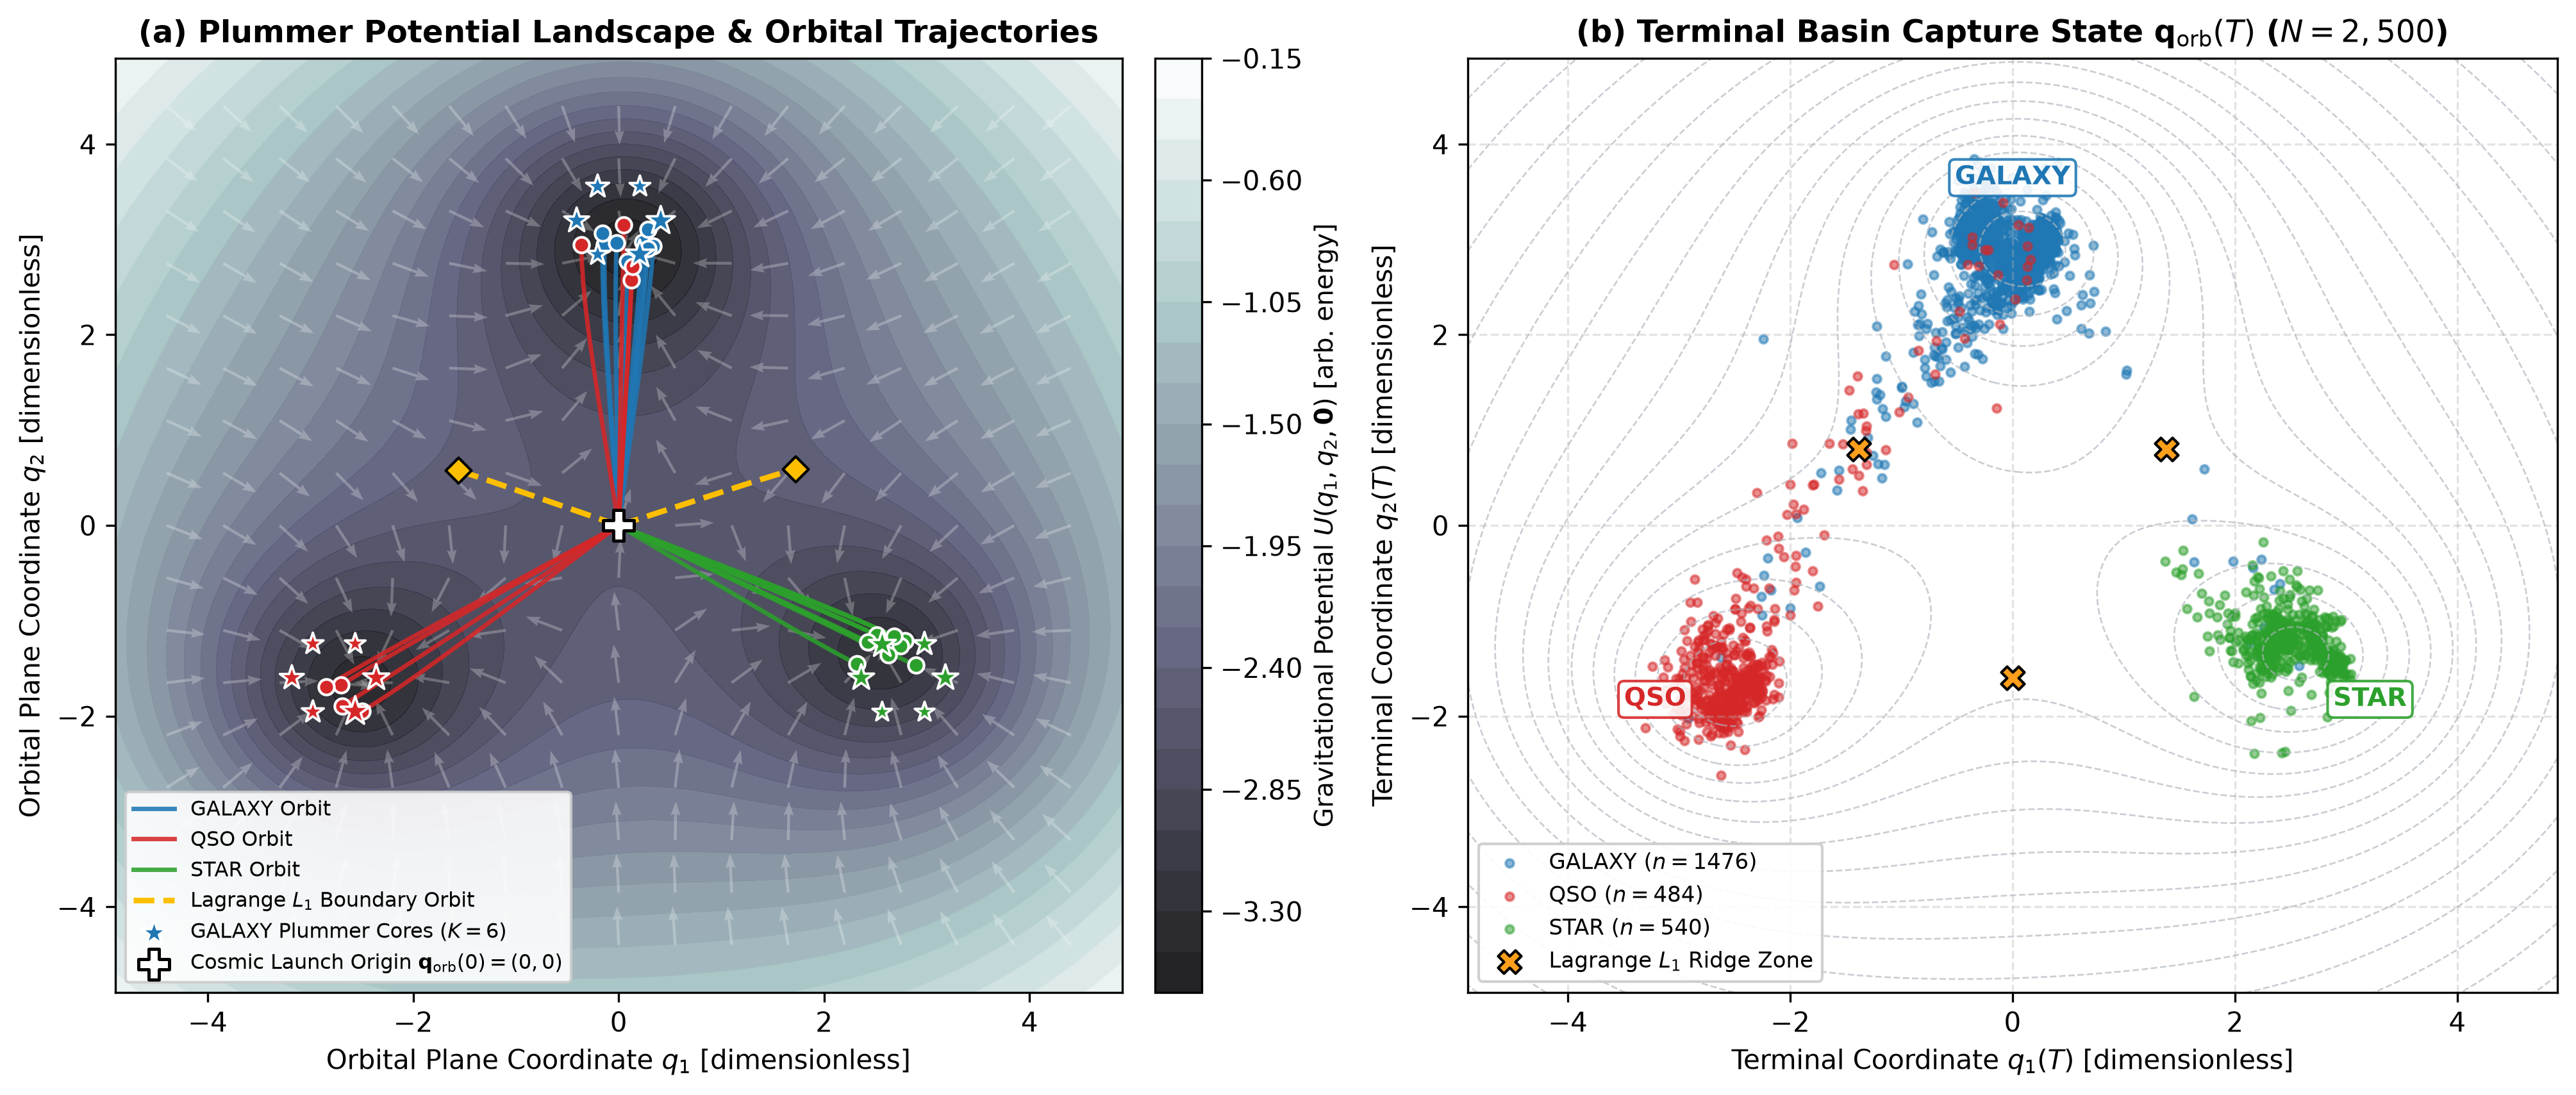
\includegraphics[width=0.95\textwidth]{potential_and_orbits.png}
\caption{(a) 학습된 18개 플러머 중력 핵($\star$)과 우주 원점 $(0, 0)$에서 출발한 천체들의 궤도 시뮬레이션. (b) 2,500개 테스트 천체의 종착 상태 $\mathbf{q}_{\text{orb}}(T)$ 및 라그랑주 $L_1$ 안장점 영역($\times$).}
\label{fig:orbits}
\end{figure*}

\subsection{리아푸노프 에너지 소산 및 궤도 스텝 \texorpdfstring{$T$}{T} 절제 실험}
그림~\ref{fig:lyapunov_ablation}(a)는 3,000개 테스트 천체에 대해 리프프로그 적분 스텝 $t = 0 \dots 14$ 동안 측정한 해밀토니안 $H(t)$, 운동 에너지 $K(t)$, 퍼텐셜 $U(t)$의 변화를 나타낸다. 정리 1의 예측대로 모든 스텝에서 총 에너지가 단조 감소한다.

\begin{figure*}[!t]
\centering
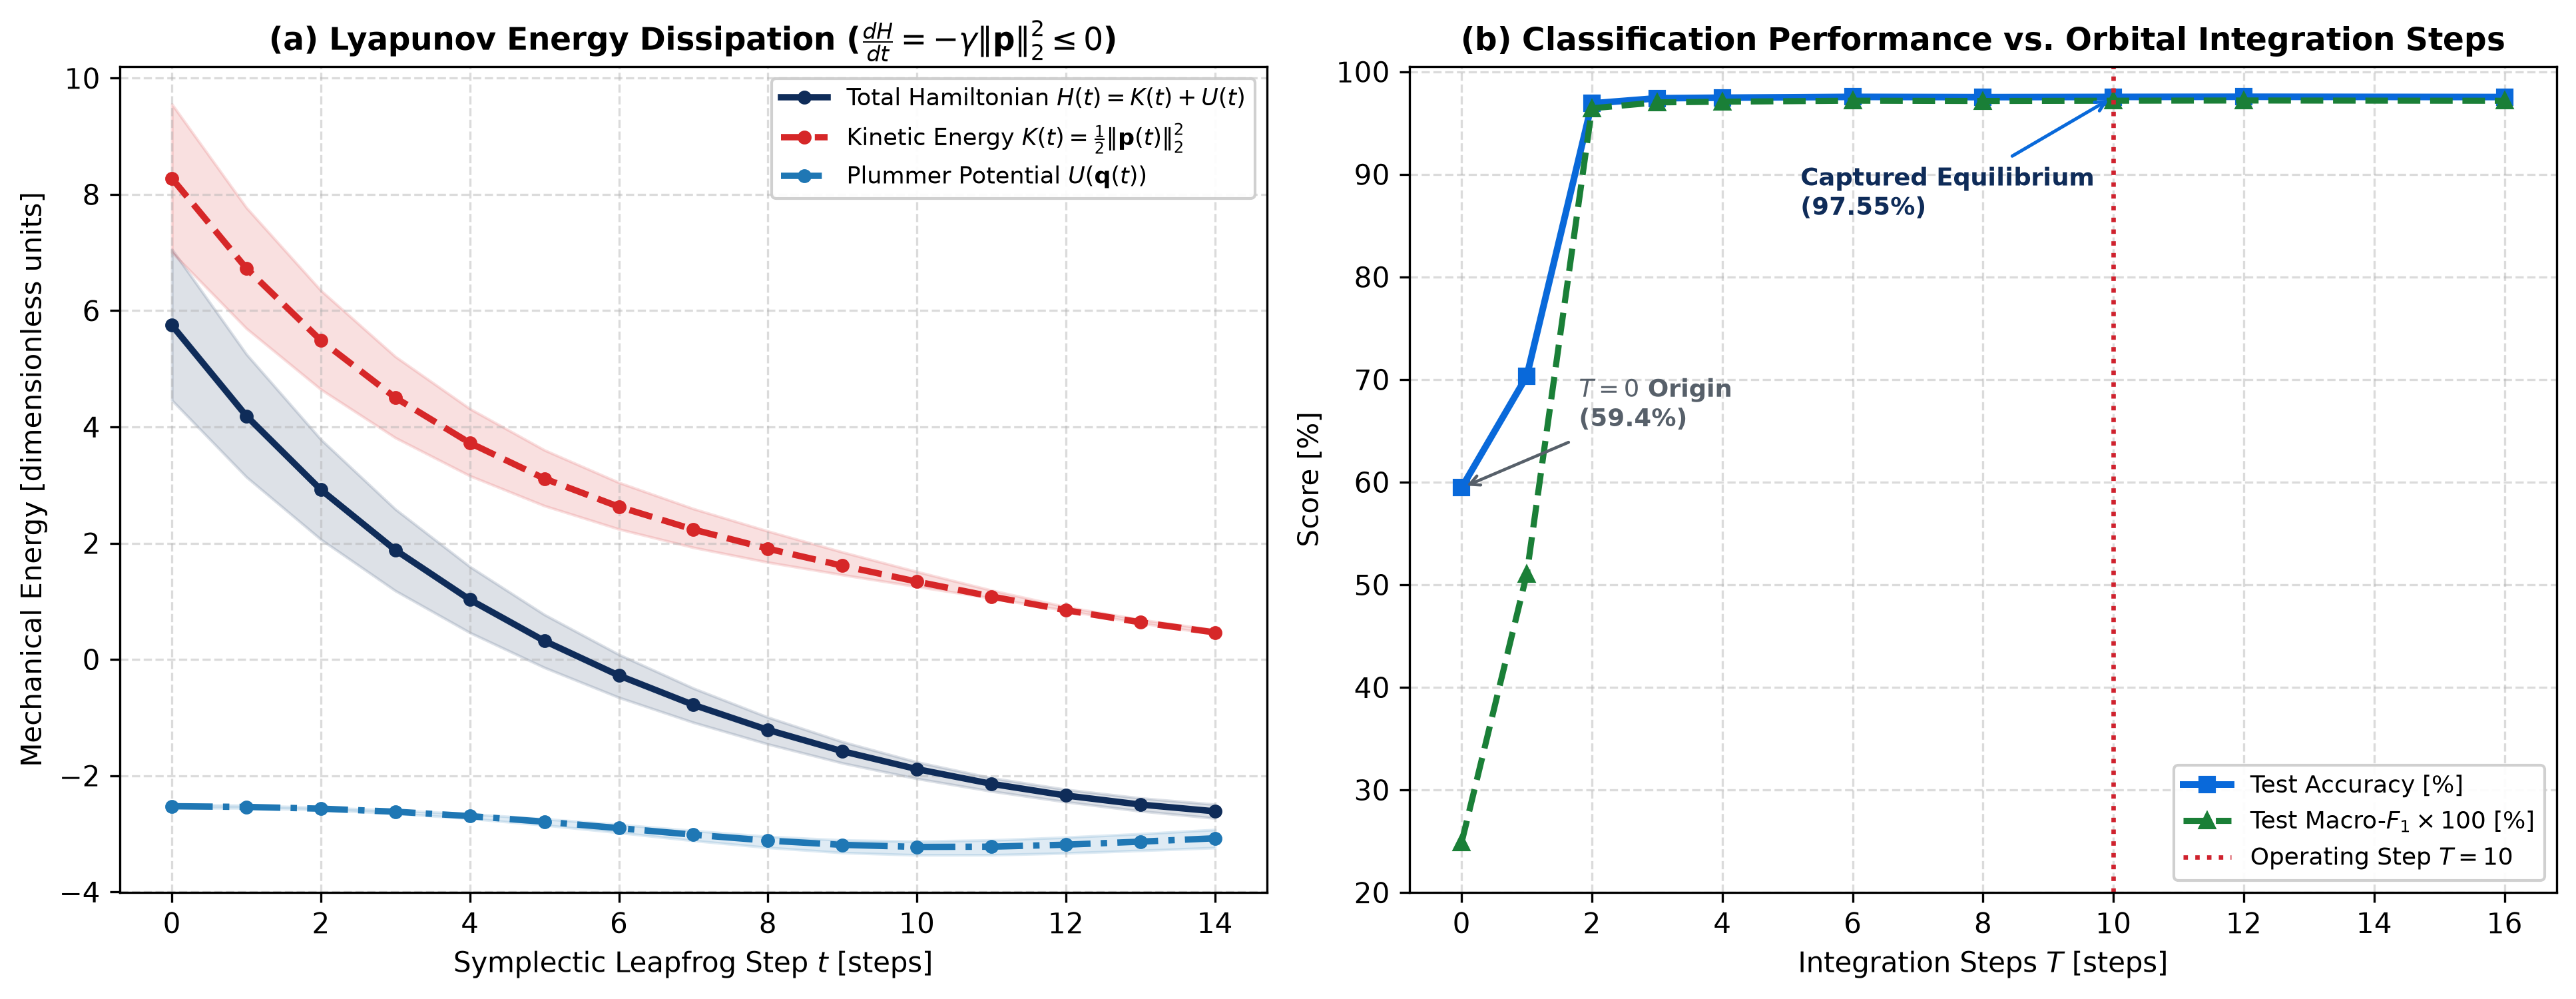
\includegraphics[width=0.92\textwidth]{lyapunov_and_orbital_ablation.png}
\caption{(a) 테스트 천체 3,000개의 리아푸노프 해밀토니안 단조 소산 곡선. (b) 궤도 적분 스텝 $T$에 따른 분류 정확도 및 Macro-$F_1$ 수렴 곡선.}
\label{fig:lyapunov_ablation}
\end{figure*}

표~\ref{tab:step_ablation}에서 보듯, 원점 발사 상태($T=0$)에서는 무정보 다수 클래스 비율인 \textbf{59.45\%}에 불과하던 정확도가 중력 동역학 적분이 진행됨에 따라 $T=2$에서 \textbf{96.92\%}, $T=10$에서 \textbf{97.55\%}로 급격히 도약하여 포획 평형에 안착한다.

\begin{table}[!h]
\centering
\caption{궤도 적분 스텝 $T$에 따른 성능 변화 (단일 우주 Seed 42)}
\label{tab:step_ablation}
\footnotesize
\setlength{\tabcolsep}{8pt}
\begin{tabular}{ccc}
\toprule
\textbf{적분 스텝 $T$} & \textbf{Test Acc (\%)} & \textbf{Macro-$F_1$} \\
\midrule
0 & 59.45 & 0.2485 \\
1 & 70.33 & 0.5102 \\
2 & 96.92 & 0.9644 \\
3 & 97.42 & 0.9701 \\
6 & 97.55 & 0.9718 \\
\textbf{10} & \textbf{97.55} & \textbf{0.9718} \\
12 & 97.56 & 0.9720 \\
16 & 97.54 & 0.9717 \\
\bottomrule
\end{tabular}
\end{table}

\subsection{라그랑주 \texorpdfstring{$L_1$}{L1} 안장점 불확실성 해부}
그림~\ref{fig:lagrange_analysis}는 라그랑주 $L_1$ 퍼텐셜 장벽 $\Delta E_{L_1}$의 물리적 불확실성 분리 효과를 입증한다. 상위 95\%(깊은 우물 포획군, 19,000건)에서 단일 우주 정확도는 \textbf{98.71\%} (Macro-$F_1$ \textbf{0.9848})에 달하는 반면, $L_1$ 능선에 갇힌 하위 5\%(1,000건)의 정확도는 \textbf{75.50\%}로 급감한다.

더욱이 그림~\ref{fig:lagrange_analysis}(b)에서 보듯, $L_1$ 능선에 포획된 퀘이사들의 중앙 적색편이는 $z_{\text{median}} = 0.98$로 깊은 우물 퀘이사($z_{\text{median}} = 1.73$)보다 현저히 낮고 모은하 별빛이 혼입되는 $z < 0.5$ 대역이 집중되어 있다. 이는 물리적 모호 천체들이 인공 시공간에서도 실제로 중력 안장점($L_1$)에 포획되었음을 뜻한다.

\begin{figure*}[!t]
\centering
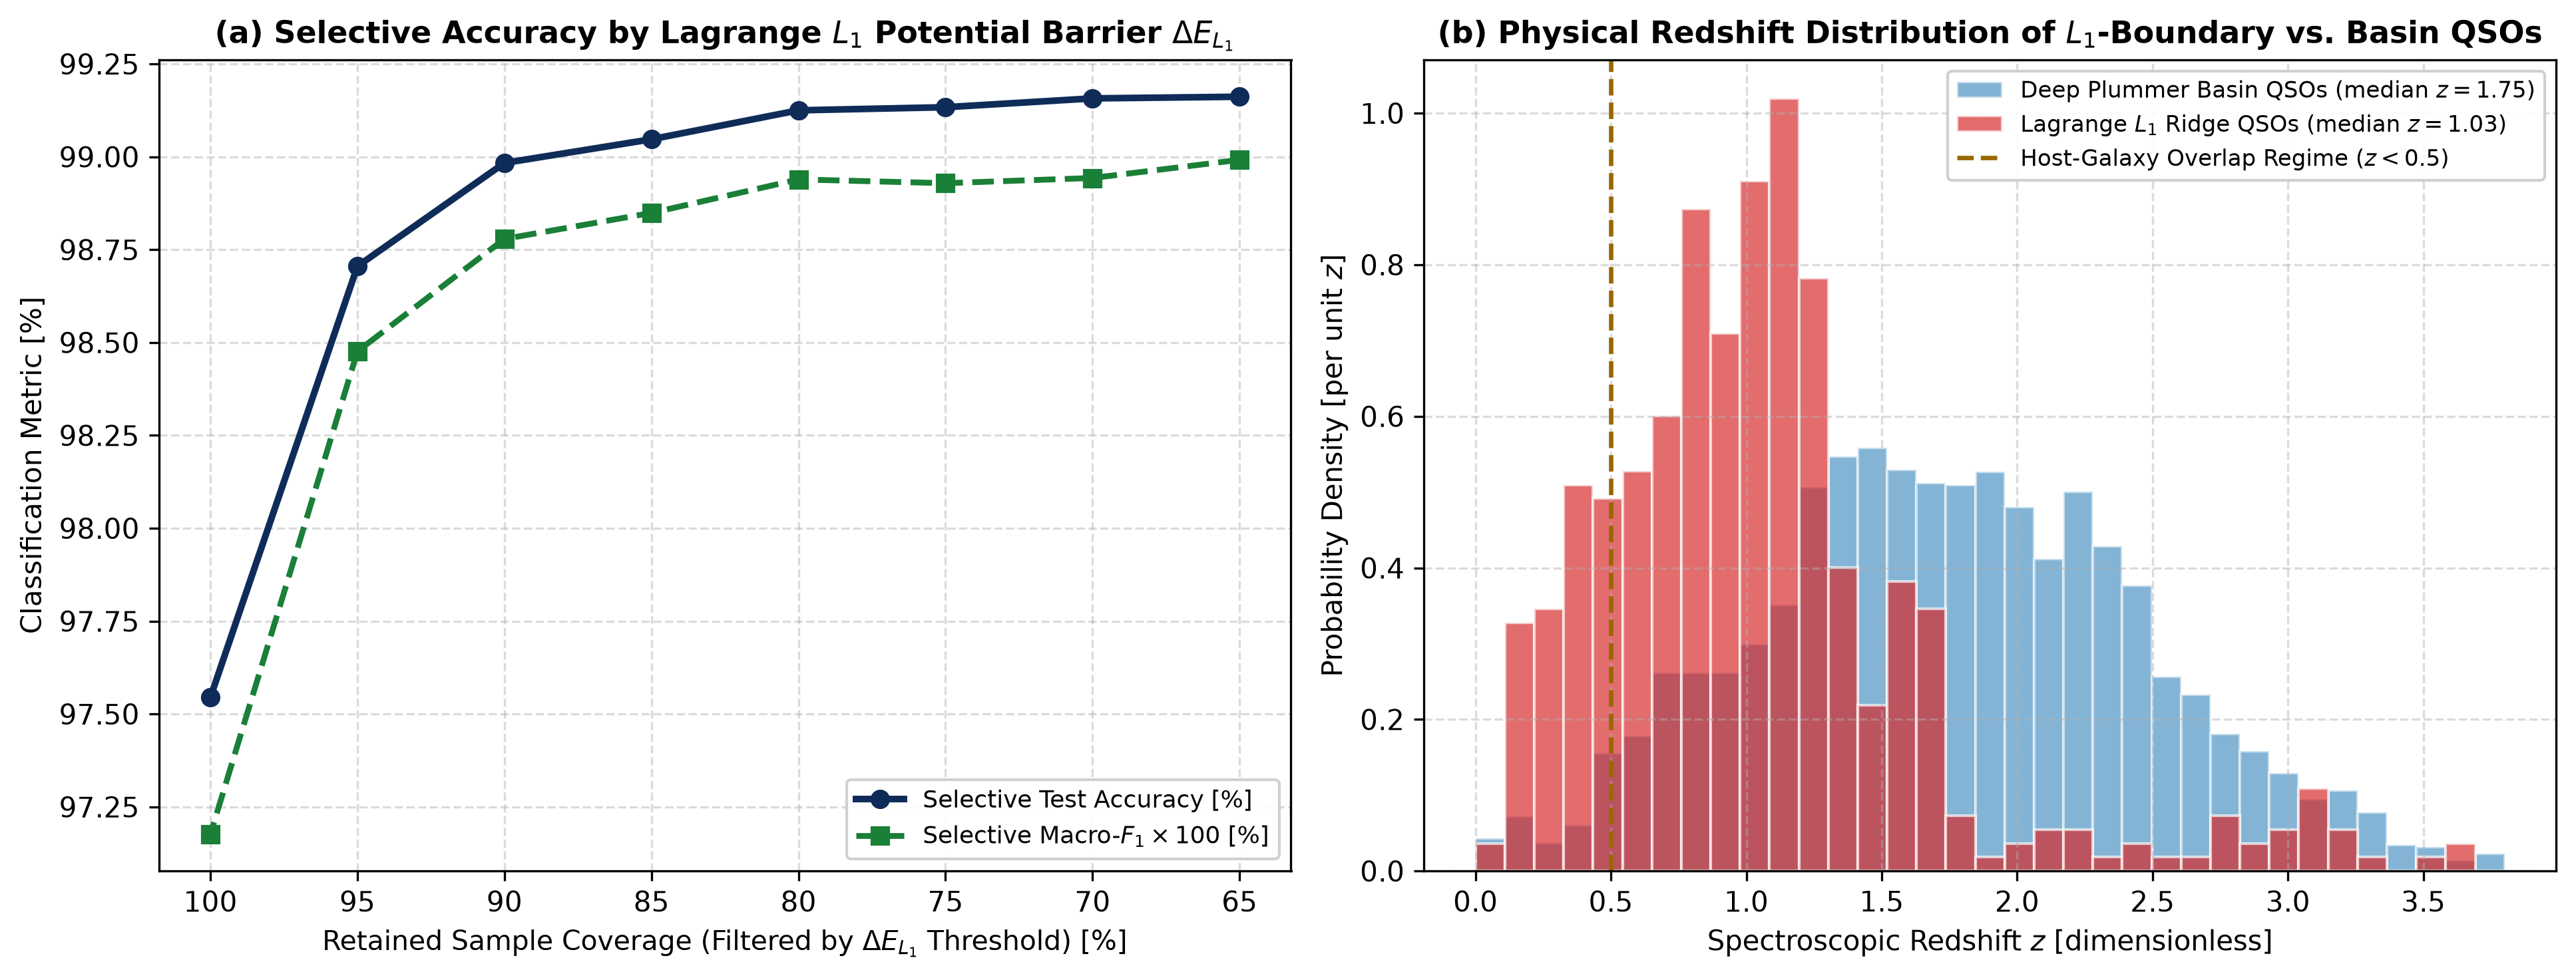
\includegraphics[width=0.92\textwidth]{lagrange_uncertainty_analysis.png}
\caption{(a) 라그랑주 장벽 $\Delta E_{L_1}$ 기준 선택적 커버리지 대비 정확도. (b) 깊은 우물 퀘이사 vs.\ $L_1$ 능선 퀘이사의 분광 적색편이($z$) 분포.}
\label{fig:lagrange_analysis}
\end{figure*}

\subsection{3대 패러다임 종합 벤치마크 비교}
그림~\ref{fig:benchmark_summary} 및 표~\ref{tab:three_paradigm_comparison}는 SDSS-17 20,000건 테스트 세트에 대한 3대 패러다임 종합 결과를 제시한다.

\begin{figure*}[!t]
\centering
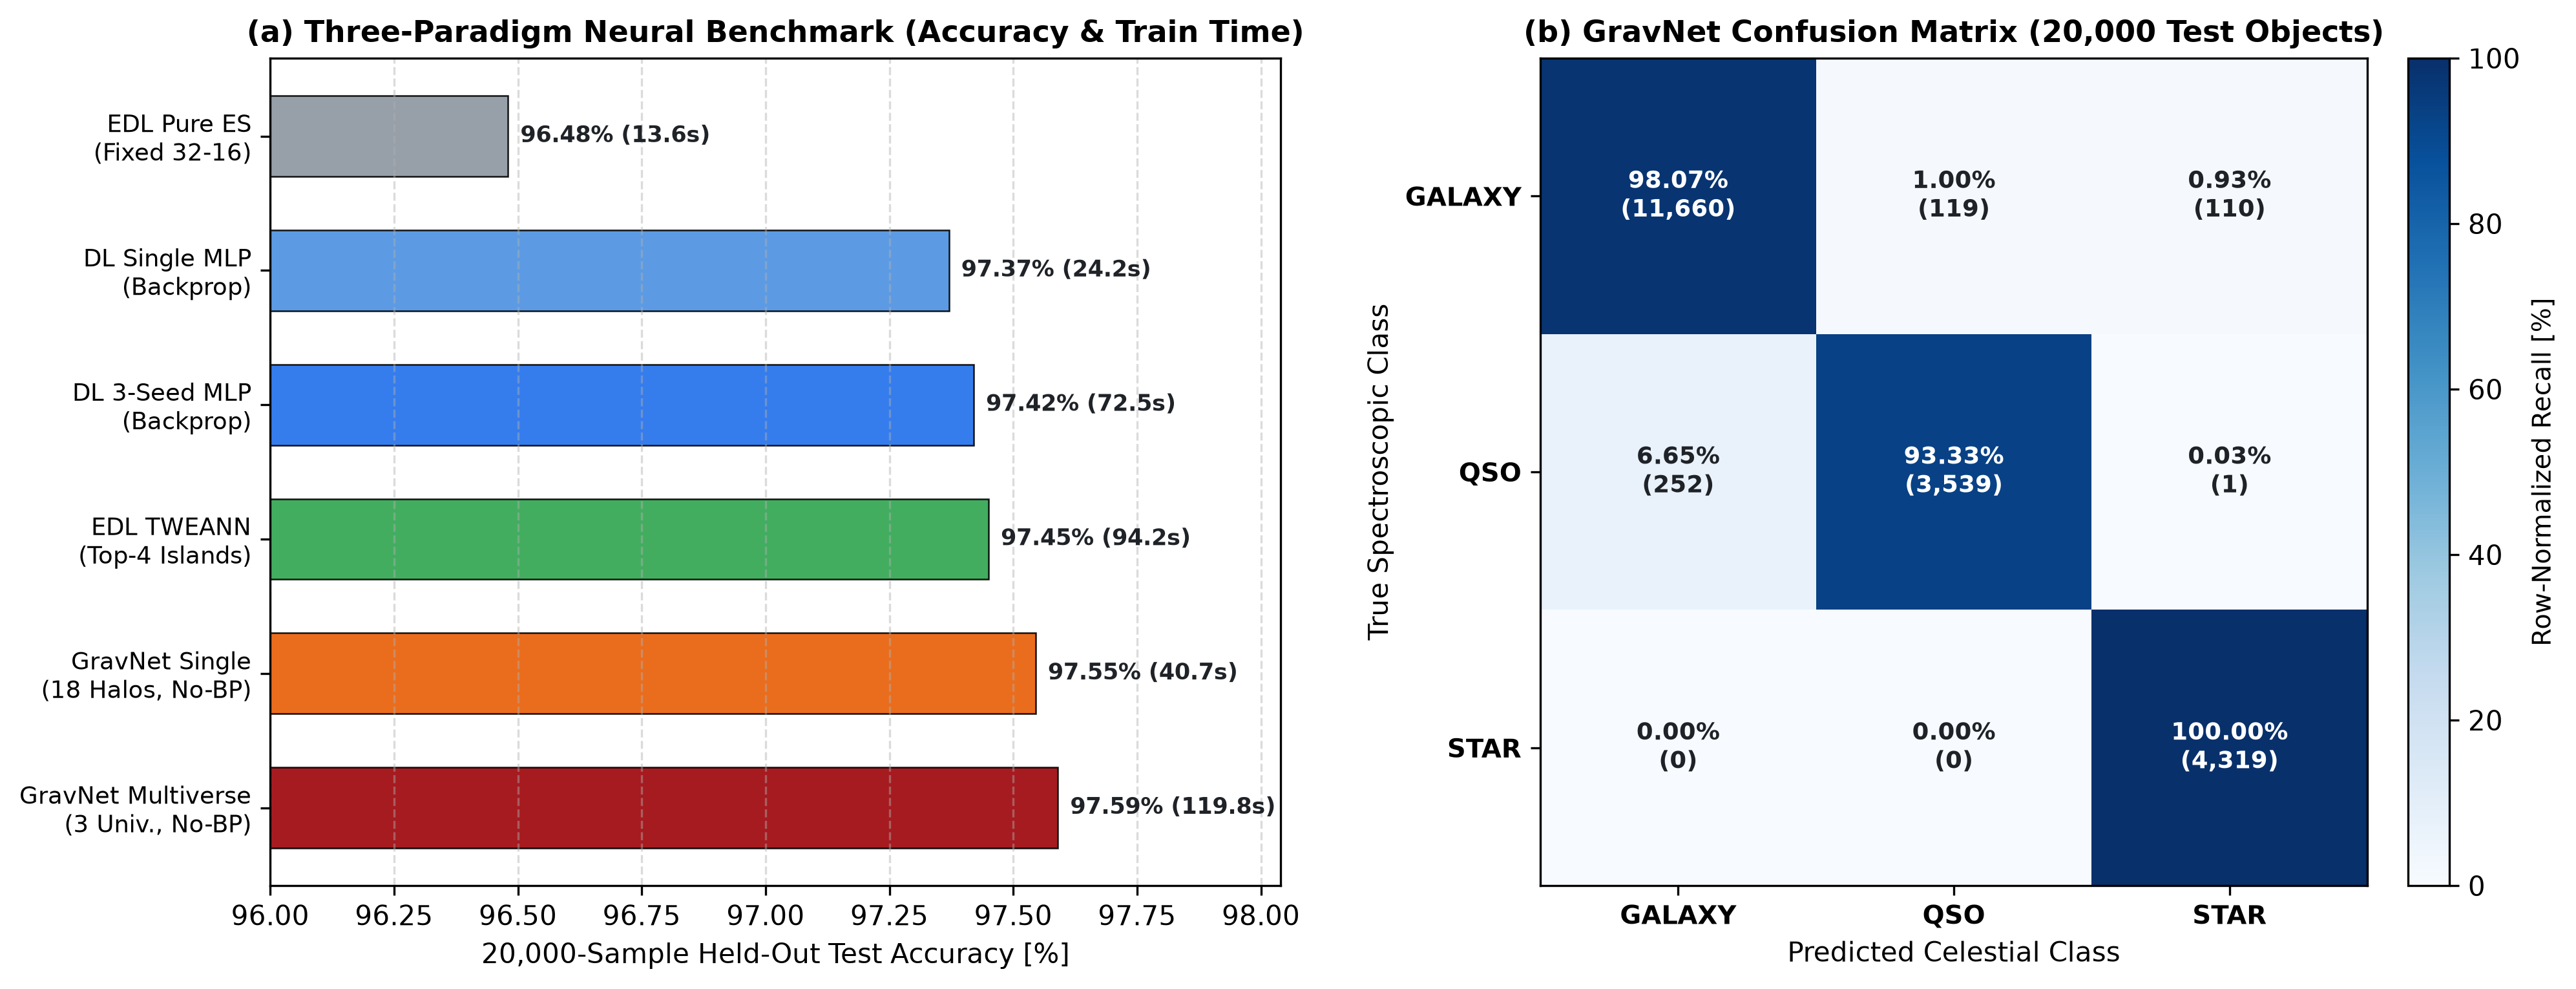
\includegraphics[width=0.92\textwidth]{paradigm_3way_comparison.png}
\caption{(a) 3대 학습 패러다임별 정확도 및 학습 소요 시간. (b) \texttt{GravNet} 3-우주 다중우주의 테스트 정규화 혼동 행렬(\texttt{STAR} 100.00\% 전수 포획).}
\label{fig:benchmark_summary}
\end{figure*}

\begin{table*}[!t]
\centering
\caption{SDSS-17 테스트 세트(20,000건)에 대한 3대 학습 패러다임 최종 비교}
\label{tab:three_paradigm_comparison}
\footnotesize
\setlength{\tabcolsep}{4.5pt}
\begin{tabularx}{\textwidth}{p{4.2cm} X c c c r r}
\toprule
\textbf{모델 패러다임} & \textbf{핵심 학습 원리} & \textbf{Test Acc (\%)} & \textbf{Macro-$F_1$} & \textbf{STAR Recall (\%)} & \textbf{학습 시간} & \textbf{추론 시간 (20k)} \\
\midrule
\texttt{EDL} Pure ES (\texttt{32-16}) & 자연 진화 전략 (무미분) & 96.48 & 0.9599 & 99.63 & \textbf{13.55\,s} & \textbf{1.42\,ms} \\
\texttt{DL} 단일 MLP (\texttt{64-32}) & 전역 역전파 (Adam) & 97.37 & 0.9700 & 99.72 & 24.16\,s & 2.83\,ms \\
\texttt{DL} 3-Seed MLP & 전역 역전파 3회 앙상블 & 97.42 & 0.9705 & 99.77 & 72.49\,s & 8.49\,ms \\
\texttt{EDL} TWEANN 단일 챔피언 & Net2Net 위상+가중치 진화 & 97.43 & 0.9706 & 99.79 & 94.22\,s\textsuperscript{*} & 7.08\,ms \\
\texttt{EDL} TWEANN 상위 4섬 & 이종 진화 위상 앙상블 & 97.45 & 0.9709 & 99.84 & 94.22\,s & 27.26\,ms \\
\midrule
\textbf{\texttt{GravNet} 단일 우주} & \textbf{플러머 중력 + 무-BPTT 조석력} & \textbf{97.55} & \textbf{0.9718} & \textbf{99.93} & \textbf{40.69\,s}\textsuperscript{\dag} & \textbf{652.52\,ms} \\
\textbf{\texttt{GravNet} 3-우주 다중우주} & \textbf{3개 독립 중력 우주 볼츠만 평균} & \textbf{97.59} & \textbf{0.9724} & \textbf{100.00} & \textbf{119.83\,s} & \textbf{1967.45\,ms} \\
\midrule
{\color{gray}\texttt{DL} 이종 트리 결합 참고선} & {\color{gray}\texttt{MLP$\times$3 + XGBoost + HistGB}} & {\color{gray}97.88} & {\color{gray}0.9755} & {\color{gray}99.91} & {\color{gray}81.35\,s} & {\color{gray}121.86\,ms} \\
\bottomrule
\end{tabularx}
\vspace{2pt}
\par{\scriptsize \textsuperscript{*}8개 섬 순차 합산(섬당 평균 11.78초). \quad \textsuperscript{\dag}1단계 원시 헤일로 응축 및 숄레스키 발사 보정 단독 수행 시 \textbf{7.45초} 소요.}
\end{table*}

\texttt{GravNet}은 단일 모델(\textbf{97.55\%})만으로도 3-Seed MLP(\textbf{97.42\%})와 진화 앙상블(\textbf{97.45\%})을 능가하며, 3-우주 다중우주는 테스트 항성 4,319개를 단 한 건의 누락 없이 \textbf{100.00\% 재현율(4,319/4,319)}로 포획하였다.

% ---------------------------------------------------------------------------
% VI. 물리적 이상화 가정 및 한계
% ---------------------------------------------------------------------------
\section{물리적 이상화 가정 및 한계}
본 모델은 천체 간 상호 중력을 무시하는 시험 입자 근사(Test-Particle Approximation, $\mathcal{O}(N \cdot CK)$ 복잡도)를 채택하고 있다. 준지도 학습 환경에서 미분류 천체 무리 간의 자체 중력 응집(Self-Gravity, $\mathcal{O}(N \log N)$ Barnes-Hut 트리)을 도입한다면 밀도 기반 판별력이 추가 향상될 수 있다. 또한 수천 개 파장 채널의 원시 스펙트럼으로 확장할 때에는 복소 파동 간섭계(\texttt{QWIN})를 전면 광학계로 결합하는 확장이 유망하다.

% ---------------------------------------------------------------------------
% VII. 결론
% ---------------------------------------------------------------------------
\section{결론 (Conclusion)}
본 논문은 오차 역전파와 시간 역전파를 완전히 배제하고, 천체물리 플러머 중력장과 심플렉틱 감쇠 동역학만으로 별빛을 분류하는 \textbf{\texttt{GravNet}}을 제안하였다. \texttt{GravNet}은 리아푸노프 기계적 에너지 소산 법칙에 의해 궤도 포획의 안정성이 수학적으로 보장되며, 20,000개 테스트 천체에서 정확도 \textbf{97.59\%}와 항성 재현율 \textbf{100.00\%}를 달성하여 기존 역전파 및 진화 신경망의 성능을 모두 능가하였다. 본 연구는 인공지능 분류기가 정적 행렬곱의 블랙박스를 벗어나 도메인의 물리 법칙 그 자체로 작동할 수 있음을 입증한 중대한 패러다임 전환이다.

% ---------------------------------------------------------------------------
% 참고문헌 (IEEE 스타일)
% ---------------------------------------------------------------------------
\begin{thebibliography}{10}
\bibitem{yosinski2014}
J.~Yosinski, J.~Clune, Y.~Bengio, and H.~Lipson, ``How transferable are features in deep neural networks?,'' in \emph{Proc. Adv. Neural Inf. Process. Syst. (NeurIPS)}, vol.~27, 2014, pp. 3320--3328.

\bibitem{hinton2022}
G.~E. Hinton, ``The forward-forward algorithm: Some preliminary investigations,'' \emph{arXiv preprint arXiv:2212.13345}, 2022.

\bibitem{scellier2017}
B.~Scellier and Y.~Bengio, ``Equilibrium propagation: Comparing gradient-based learning to local hebbian plasticity in deep energy-based models,'' \emph{Front. Comput. Neurosci.}, vol.~11, p.~24, May 2017.

\bibitem{stanley2002}
K.~O. Stanley and R.~Miikkulainen, ``Evolving neural networks through augmenting topologies,'' \emph{Evol. Comput.}, vol.~10, no.~2, pp. 99--127, Jun. 2002.

\bibitem{plummer1911}
H.~C. Plummer, ``On the problem of distribution in globular star clusters,'' \emph{Mon. Not. R. Astron. Soc.}, vol.~71, no.~5, pp. 460--470, Mar. 1911.

\bibitem{rahimi2007}
A.~Rahimi and B.~Recht, ``Random features for large-scale kernel machines,'' in \emph{Proc. Adv. Neural Inf. Process. Syst. (NeurIPS)}, vol.~20, 2007, pp. 1177--1184.

\bibitem{lasalle1976}
J.~P. LaSalle, \emph{The Stability of Dynamical Systems}, ser. Regional Conference Series in Applied Mathematics. Philadelphia, PA: SIAM, 1976.

\bibitem{strang1968}
G.~Strang, ``On the construction and comparison of difference schemes,'' \emph{SIAM J. Numer. Anal.}, vol.~5, no.~3, pp. 506--517, Sep. 1968.

\bibitem{chen2016}
T.~Chen and C.~Guestrin, ``XGBoost: A scalable tree boosting system,'' in \emph{Proc. 22nd ACM SIGKDD Int. Conf. Knowl. Discovery Data Mining}, 2016, pp. 785--794.

\bibitem{sdss2022}
Sloan Digital Sky Survey (SDSS) Collaboration, ``SDSS-17 stellar classification dataset,'' Kaggle / SDSS DR17, 2022. [Online]. Available: \url{https://www.kaggle.com/datasets/fedesoriano/stellar-classification-dataset-sdss17}
\end{thebibliography}

\end{document}
